\clearpage
\section{Optical flow sensor}

An Optical flow sensor uses a camera to detect motion on a the x and y plane. It looks for movement by finding patterns on the ground to be able to determine the direction it is travelling in and how far the sensor has moved. This is vital information for SLAM mapping, since it is necessary to know where the mapping devices is placed compared to previous measurements, this means that the optical flow sensor is used for finding the reference points. The sensor should be mounted quite high above ground on the rover to get a bigger view of the ground area, and is faced downwards to the ground.

The optical flow sensor works in the same manner as a computer mouse and gives back information to the rover. What is important is the surface that the optical flow is looking at. If it is reflective or has many differences that the camera can use for reference, the readings will be wrong incorrect. It is therefore good to have a backup system to ensure that the rover receives a correct reference point, like encoders on the wheels so the program knows that the rover is moving.


\begin{figure}[H]
	\centering
	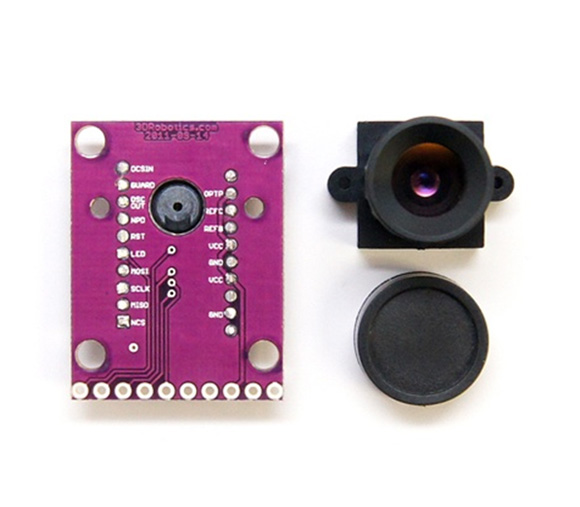
\includegraphics[width=.3\linewidth]{images/optical.jpg}
	\caption{The optical flow sensor from 3D Robotics.}
\end{figure}


%cite http://en.wikipedia.org/wiki/Optical_flow